\documentclass[twoside,11pt]{article}

\usepackage{jmlr2e}
\usepackage{amsmath}
\usepackage{microtype}
\usepackage{booktabs}
\usepackage{tabularx}
\usepackage{array}
\usepackage{enumitem}
\usepackage{lastpage}
\usepackage{tikz}
\usetikzlibrary{positioning,calc,arrows.meta}

\jmlrheading{0}{2026}{1-\pageref{LastPage}}{Submitted 5/2026}{Preprint}{PAPER-BC-0001}{Jonathan Herrera-Vasquez}
\ShortHeadings{XAI Metrics: Taxonomy and LIME--SHAP Comparison}{Herrera-Vasquez}
\firstpageno{1}

\begin{document}

\title{From Fidelity to Semantics:\\
A Taxonomy of XAI Evaluation Metrics\\
and Paired Empirical Comparison of LIME versus SHAP}

\author{
\name Jonathan Herrera-Vasquez \email jonnabio@gmail.com \\
\addr Universidad Americana de Europa (UNADE)\\
Canc\'un, Quintana Roo, M\'exico
}

\editor{}

\maketitle

\begin{abstract}
Evaluation of post-hoc explanations in machine learning remains fragmented
across incompatible metric families, yielding method comparisons that are
sensitive to which endpoints are chosen. We address this through two
complementary contributions. First, drawing on 48 coded papers from a five-database structured
search with PRISMA-style screening, we build a four-axis taxonomy---by
evaluation target, evidence source, quality property, and task
context---that maps the measurement landscape and exposes three recurring
gaps: proxy metrics dominate despite not
capturing semantics; human-grounded constructs remain underspecified; and
semantic evaluation is growing faster than its empirical validation base.
Second, we fill the proxy-layer gap with a paired empirical benchmark
comparing LIME and SHAP across 75 matched cells spanning five model
families, five seeds, and three sampling sizes on tabular data. Results
are consistent and large in magnitude: SHAP dominates all quality
endpoints (stability $d_z{=}3.00$, fidelity $d_z{=}4.82$, faithfulness
gap $d_z{=}2.63$), while LIME is faster for non-tree model families
(median 53.3 ms vs.\ 694.6 ms for SHAP); for tree-based models, SHAP's
\texttt{TreeExplainer} reverses this ordering. Cross-dataset replication
on two additional datasets confirms SHAP's fidelity advantage over Anchors
in all 12 paired combinations. Together, the taxonomy and the benchmark
motivate a model-architecture-conditioned deployment pattern: SHAP is
preferred at both fidelity and latency for tree-based models, while LIME
retains a latency advantage for black-box architectures lacking a
model-aware explainer. All experimental artifacts are publicly available.
\end{abstract}

\begin{keywords}
explainable AI, evaluation metrics, taxonomy, LIME, SHAP
\end{keywords}

% -----------------------------------------------------------------------
\section{Introduction}
\label{sec:intro}
% -----------------------------------------------------------------------

Selecting an explanation method in production can be posed as a
constrained decision problem: given a fixed predictor $f$ and instance
$x$, choose $E \in \{\mathrm{LIME}, \mathrm{SHAP}\}$ to maximize
explanation quality while satisfying operational constraints. Concretely,
we consider
\[
E^\star = \arg\max_{E \in \{\mathrm{LIME},\mathrm{SHAP}\}}
U(S_E, F_E, \Delta_{k,E}, P_E)
\quad\text{s.t.}\quad C_E \le \tau,
\]
where $S$ is stability, $F$ fidelity, $\Delta_k$ faithfulness gap, $P$
sparsity, $C$ cost, and $\tau$ a latency budget. Yet this decision
problem cannot be resolved in the abstract: it requires an organizing
framework that identifies which quality properties matter, what evidence
supports their measurement, and where structural proxy metrics end and
semantic or human-centered evaluation begins.

Progress in explainable AI (XAI) depends on evaluating whether
explanations are useful, faithful, stable, and meaningful. Yet the
literature does not converge on a single definition of explanation
quality. Surveys consistently note that XAI evaluation is fragmented
across proxy metrics, qualitative user studies, and domain-specific
desiderata \citep{adadi2018xai,arrieta2020xai,kadir2023metrics,
canha2025benchmark}. As a result, comparisons between explainers often
depend as much on the chosen metric family as on the methods themselves.

\begin{sloppypar}
This fragmentation is especially visible in model-agnostic post-hoc
explainability. Faithfulness-style metrics remain common because they are
relatively easy to compute, but they do not fully capture whether an
explanation is understandable, semantically aligned with domain knowledge,
or decision-useful in practice
\citep{ali2023trustworthy,longo2024manifesto}.
Multi-metric work shows that stability, sparsity, and cost are also
part of explanation quality, and recent analyses confirm that distinct
metrics reveal complementary signals \citep{pawlicki2024metrics,zheng2025ffidelity}.
\end{sloppypar}

LIME and SHAP are the most widely deployed model-agnostic post-hoc
explainers for tabular data, yet their systematic multi-metric comparison
under controlled conditions remains scarce. \citet{retzlaff2024posthoc} survey post-hoc versus ante-hoc design
guidelines and review method properties, but do not provide matched
empirical benchmarks across model families, metrics, and sampling regimes;
this paper fills that gap. LIME explains locally by
fitting a sparse surrogate around $x$:
\[
\xi(x) = \arg\min_{g \in G} \mathcal{L}(f, g, \pi_x) + \Omega(g),
\]
favoring local fidelity and explicit sparsity controls
\citep{ribeiro2016why}. SHAP explains predictions through additive
feature attributions $f(x) = \phi_0 + \sum_i \phi_i$, where $\phi_i$
are Shapley-based contributions with game-theoretic guarantees
\citep{lundberg2017unified}. Their theoretical differences are well
known, but do not by themselves resolve deployment choices across model
families, sampling regimes, and runtime constraints
\citep{retzlaff2024posthoc,ali2023trustworthy}.

This paper makes five contributions:
\begin{enumerate}[leftmargin=*]
\item \textbf{Four-axis taxonomy}: we organize model-agnostic XAI
evaluation along evaluation target, evidence source, quality property,
and task context, making explicit why metric disagreements arise.
\item \textbf{Gap analysis}: from a documented corpus of 48 papers
(five databases, PRISMA-style screening) we identify three systematic
gaps---proxy dominance, underspecified human constructs, and semantic
evaluation outpacing its validation base---and provide, to our
knowledge, the first multi-rater LLM-judge reliability measurement in
XAI (ICC$<$0.75 across all seven semantic dimensions).
\item \textbf{Formalized deployment decision}: we pose LIME-vs-SHAP
selection as a constrained multi-objective problem over quality, parsimony,
and cost.
\item \textbf{Paired inferential evidence}: we quantify method differences
on 75 matched cells with Holm-corrected significance testing and effect
sizes for five endpoints, and replicate fidelity rankings across two
additional datasets via cross-dataset validation (EXP3).
\item \textbf{Layered deployment architecture}: we derive deployment
recommendations from both the taxonomy and the empirical results, mapping
system constraints to explainer choice.
\end{enumerate}

% -----------------------------------------------------------------------
\section{Background and Definitions}
\label{sec:background}
% -----------------------------------------------------------------------

To keep the taxonomy and benchmark precise, we first separate several
terms that are frequently conflated in XAI writing.

\subsection{Intrinsic versus Post-Hoc Explainability}

Intrinsic models are designed to be interpretable by construction, whereas
post-hoc methods attempt to explain black-box behavior after training
\citep{rudin2019stop,retzlaff2024posthoc}. This survey and benchmark focus
exclusively on post-hoc model-agnostic explainability, which is the dominant
paradigm for tabular ML deployments. Metric validity conditions for
intrinsic models differ substantially and are out of scope here.

\subsection{Explanation Quality versus Model Quality}

A model may be accurate while producing unstable or semantically weak
explanations; conversely, a model can support concise explanations without
being more accurate. Evaluation therefore needs to specify whether the
object under study is the explanation artifact, the explainer method, the
predictive model, or the user-facing decision process. Conflating these
levels produces inconsistent benchmark conclusions.

\subsection{Local versus Global Explanations}

Local attributions and counterfactuals are typically judged through
faithfulness, sparsity, or actionability. Global summaries may be judged
by coverage, consistency, or conceptual coherence. Many reported metric
disagreements arise because local and global levels are mixed without
explicit task framing. This paper focuses on local post-hoc explanations.

\subsection{Semantic versus Structural Evaluation}

A structural proxy metric such as perturbation faithfulness evaluates
whether feature rankings track model sensitivity under a chosen intervention.
A semantic judgment evaluates whether an explanation ``makes sense'' under
domain, causal, or linguistic criteria. Both matter for deployment decisions,
but they are not interchangeable; substituting one for the other conceals
important gaps in evaluation coverage.

\subsection{LIME: Local Interpretable Model-Agnostic Explanations}

LIME approximates a black-box model $f$ locally around an instance $x$
by training an interpretable surrogate $g$ on perturbed samples weighted
by kernel $\pi_x$:
\[
\xi(x) = \arg\min_{g \in G} \mathcal{L}(f, g, \pi_x) + \Omega(g),
\]
where $\Omega(g)$ penalizes complexity \citep{ribeiro2016why}. LIME
behavior is strongly shaped by neighborhood construction hyperparameters
(kernel width, perturbation sample count, feature budget). These controls
yield compact explanations and low latency, but they introduce stochastic
variation because local neighborhoods are sampled rather than exhaustively
enumerated.

\subsection{SHAP: Shapley Additive Explanations}

SHAP attributes prediction output to features based on marginal
contribution across all possible coalitions, satisfying efficiency,
symmetry, and dummy axioms \citep{lundberg2017unified}. KernelSHAP
estimates Shapley values with a weighted regression scheme over coalitions
for model-agnostic use; tree-specific implementations exploit model
structure for speed. Relative to local-surrogate methods, SHAP is
typically denser and computationally heavier in non-tree settings because
many coalition evaluations are required.

\subsection{Benchmark Design Implications}

For a fair LIME-versus-SHAP comparison, confounders unrelated to explainer
design must be controlled. This motivates the protocol choices in
Section~\ref{sec:empirical}: identical transformed feature space, shared
model artifacts, fixed class target, and matched cells by
$(\mathrm{model}, \mathrm{seed}, N)$. Under these controls, expected
methodological trade-offs become testable: LIME should favor sparsity and
speed, while SHAP should favor stability and faithfulness. This framing
aligns with calls for multi-metric, functionally grounded XAI evaluation
\citep{pawlicki2024metrics,canha2025benchmark}.

% -----------------------------------------------------------------------
\section{Taxonomy of XAI Evaluation Metrics}
\label{sec:taxonomy}
% -----------------------------------------------------------------------

The central contribution of this section is that XAI evaluation can be
clarified by crossing four axes: evaluation target, evidence source,
quality property, and task context. Metrics that appear to answer the
same question often do not, because they attach to different objects, use
different evidence, or imply different validity conditions.

\subsection{Taxonomy by Evaluation Target}

Many metric disagreements start with a hidden mismatch about what is
being evaluated:
\begin{itemize}[leftmargin=*]
\item \textbf{Explanation artifact metrics} evaluate the produced
explanation itself---attribution sparsity, local fidelity, or semantic
clarity.
\item \textbf{Explainer method metrics} evaluate the behavior of the
explainer across cases---stability, reproducibility, or computational
cost.
\item \textbf{Model-behavior metrics} evaluate whether explanations track
model behavior under perturbations or alternative decision regions.
\item \textbf{User/task outcome metrics} evaluate whether explanations
improve decision performance, trust calibration, or actionability.
\end{itemize}

This distinction matters because one metric family cannot automatically
stand in for another. A sparse explanation can still be semantically
misleading; a faithful attribution can still be unusable in a
decision-support workflow.

\subsection{Taxonomy by Evidence Source}

The second axis concerns the evidence used to justify the evaluation:
\begin{itemize}[leftmargin=*]
\item \textbf{Proxy or perturbation metrics} infer quality from numerical
sensitivity behavior under intervention.
\item \textbf{Benchmark-grounded metrics} compare explanations to
synthetic or domain-defined ground truth.
\item \textbf{Human expert judgments} evaluate plausibility, correctness,
or domain alignment.
\item \textbf{End-user studies} assess comprehension, trust calibration,
decision quality, or cognitive load.
\item \textbf{LLM judges} provide scalable semantic scoring via
rubric-guided language-model evaluation.
\end{itemize}

Proxy metrics are scalable and reproducible but may under-capture meaning.
Human judgments are richer but expensive and variable. LLM judges are
scalable like proxies but semantically expressive like human reviews,
which is precisely why their validity must be established rather than
assumed \citep{gu2024llmjudge,wu2025userperceptions,zhou2025medthink}.
Evidence Source thus characterizes \emph{how} measurement evidence is generated---the modality of observation---while Quality Property (below) characterizes \emph{what} construct is claimed; the same quality property can in principle be assessed via multiple evidence sources, and the same source type can serve multiple properties.

\subsection{Taxonomy by Quality Property}

The literature returns repeatedly to a familiar set of quality properties,
though not always with consistent definitions:
\begin{itemize}[leftmargin=*]
\item \textbf{Fidelity / faithfulness:} whether the explanation tracks
how the model actually behaves under feature interventions or masking
\citep{ribeiro2016why,lundberg2017unified,zheng2025ffidelity}.
\item \textbf{Stability / robustness:} whether similar inputs yield
similar explanations under perturbation or reruns
\citep{pawlicki2024metrics,canha2025benchmark}.
\item \textbf{Sparsity / parsimony:} whether the explanation is concise
enough to be interpretable without unnecessary feature load.
\item \textbf{Plausibility:} whether the explanation aligns with domain
expectations or expert reasoning.
\item \textbf{Counterfactual or recourse quality:} whether
explanation-linked interventions are feasible, minimal, diverse, or
actionable \citep{mothilal2020dice}.
\item \textbf{Semantic alignment:} whether an explanation captures
meaningful causal or conceptual structure, even when proxy metrics are
agnostic to that structure.
\end{itemize}

These properties are only partly commensurable. A method can score
strongly on fidelity while remaining weak on sparsity or semantic
adequacy. Multi-metric reporting is therefore not optional; it is the
minimum needed to make XAI claims interpretable across use cases.

\begin{table}[t]
\centering
\caption{Working construct dictionary: operational meanings and strongest
direct evidence for each quality property.}
\begin{tabularx}{\linewidth}{l X X}
\toprule
\textbf{Construct} & \textbf{Operational meaning} & \textbf{Strongest evidence} \\
\midrule
Fidelity / faithfulness & Whether the explanation tracks model behavior under a specified intervention or masking scheme. & Proxy tests and benchmark-grounded checks \\
Stability / robustness & Whether explanations remain consistent across reruns, perturbations, or nearby inputs. & Proxy perturbation studies and repeated-run analyses \\
Sparsity / parsimony & Whether explanations keep feature load low enough to remain cognitively manageable. & Structural summaries of explanation size or weight concentration \\
Plausibility & Whether explanations align with expert expectations or domain logic. & Expert-human review with explicit rubrics \\
Semantic alignment & Whether explanations capture meaningful conceptual or causal structure beyond structural proxy success. & Expert review or validated semantic evaluators \\
User usefulness & Whether explanations improve comprehension, decision quality, or trust calibration in an actual task. & End-user studies with task outcomes \\
\bottomrule
\end{tabularx}
\label{tab:constructs}
\end{table}

\subsection{Taxonomy by Task Context}

Metric validity also depends on context. Tabular benchmarks often assume
feature independence, perturbation realism, and tractable local
neighborhoods. These assumptions can fail in image, text, graph, and
time-series settings, where perturbations may create out-of-distribution
examples or semantically invalid transformations
\citep{agarwal2023gnn_eval,proszewska2025bxaic}. Metric transport across
modalities cannot be assumed.

\begin{table}[t]
\centering
\caption{Core metric families in model-agnostic XAI evaluation: what
each captures well and what it leaves unresolved.}
\footnotesize
\begin{tabularx}{\linewidth}{l X X}
\toprule
\textbf{Metric family} & \textbf{Captures well} & \textbf{Leaves unresolved} \\
\midrule
Fidelity / faithfulness & Whether explanations track model behavior under interventions or masking. & Whether the explanation is meaningful, plausible, or useful outside the proxy setup. \\
Stability / robustness & Whether explanations remain consistent across perturbations or repeated runs. & Whether stable explanations are actually correct or semantically adequate. \\
Sparsity / parsimony & Whether explanations are concise and low in feature load. & Whether concision hides necessary nuance or context. \\
Benchmark-grounded correctness & Whether explanations recover synthetic or domain-defined ground truth. & Whether the ground truth is realistic, complete, or transferable. \\
Human expert review & Whether explanations align with domain expectations and expert reasoning. & Whether those judgments are scalable, standardized, and reproducible. \\
User-centered evaluation & Whether explanations improve understanding, decisions, or trust calibration in practice. & Whether findings generalize across tasks, populations, and study designs. \\
LLM-based semantic evaluation & Whether rubric-based semantic judgments can be produced quickly and at scale. & Whether those judgments agree with humans and avoid proxy-judge bias. \\
\bottomrule
\end{tabularx}
\label{tab:taxonomy_families}
\end{table}

Table~\ref{tab:taxonomy_families} illustrates the practical consequence of
the taxonomy: each metric family gains strength by focusing on one kind
of evidence and one kind of target, but each also leaves predictable
blind spots. No single family can exhaust explanation quality on its own.

% -----------------------------------------------------------------------
\section{Comparative Synthesis and Open Gaps}
\label{sec:synthesis}
% -----------------------------------------------------------------------

\subsection{Search Protocol and Corpus Profile}

\paragraph{Search strategy.}
We searched five bibliographic databases: Semantic Scholar, Google
Scholar, ACM Digital Library, IEEE Xplore, and ACL Anthology. Two
query families were applied. The primary query combined evaluation-object
terms (\emph{``explainable AI'' OR ``XAI'' OR ``interpretable machine
learning''}) with evaluation-act terms (\emph{``evaluation'' OR
``benchmark'' OR ``metric'' OR ``assessment''}). A secondary query
targeted method-comparative literature: (\emph{``LIME'' OR ``SHAP'' OR
``attribution method''}) AND (\emph{``evaluation'' OR ``stability'' OR
``fidelity''}). Both queries were restricted to English-language
publications from January 2015 to March 2026. Conference proceedings,
journal articles, and ArXiv preprints with an accompanying peer-reviewed
venue were eligible; informal workshop papers without self-contained
empirical evaluations were excluded.

\paragraph{Inclusion and exclusion criteria.}
A paper was \emph{included} if it: (i) proposes, operationalizes, or
critically analyses an evaluation metric or evaluation paradigm for
post-hoc model-agnostic explanations; (ii) provides a formal or
empirical evaluation component beyond merely applying an explainer to a
dataset; and (iii) is available in full text. A paper was \emph{excluded}
if it: focuses exclusively on intrinsic or white-box interpretability
without a metric generalizable to post-hoc settings; is a
domain-specific clinical or scientific application with no reusable
evaluation component; or contributes only to model training methodology.
Borderline cases were resolved by conservatively admitting sources
containing at least one codeable evaluation construct relevant to the
four-axis taxonomy.

\paragraph{PRISMA-style screening record.}
Table~\ref{tab:prisma} documents the staged screening. Records were
first pooled and deduplicated across databases, then screened on title
and abstract, then assessed in full text.

\begin{table}[t]
\centering
\caption{Corpus construction screening record (PRISMA-style).}
\label{tab:prisma}
\begin{tabular}{lr}
\toprule
Stage & Records \\
\midrule
Identified via database searches & 312 \\
Removed after cross-database deduplication & 65 \\
Screened on title and abstract & 247 \\
Excluded at screen (out of scope, non-English, no eval component) & 152 \\
Full text assessed for eligibility & 95 \\
Excluded at full text (intrinsic only, no codeable metric) & 47 \\
\midrule
\textbf{Included in coded corpus} & \textbf{48} \\
\bottomrule
\end{tabular}
\end{table}

\paragraph{Corpus structure.}
Each of the 48 coded papers is assigned to one or more thematic clusters
and coded along four dimensions. Inclusion requires that a source
contribute a formal evaluation construct, a benchmark design principle,
a warning about metric misuse, or an evaluation paradigm directly
relevant to post-hoc model-agnostic explanations. The coding protocol
captures four dimensions for each paper:

\begin{table}[t]
\centering
\caption{Coding dimensions used to build the taxonomy.}
\begin{tabularx}{\linewidth}{l X}
\toprule
\textbf{Dimension} & \textbf{Operational question} \\
\midrule
Evaluation target & What is being judged: explanation artifact, explainer, model behavior, or user/task outcome? \\
Evidence source & What kind of evidence supports the judgment: perturbation proxy, benchmark ground truth, human rating, user task, or LLM judge? \\
Quality property & Which property is claimed: fidelity, stability, sparsity, plausibility, recourse quality, semantic alignment? \\
Task context & In what modality or domain is the metric assumed to be meaningful? \\
\bottomrule
\end{tabularx}
\label{tab:coding_dims}
\end{table}

\begin{table}[t]
\centering
\caption{Descriptive profile of the review corpus (48 coded papers).}
\begin{tabularx}{\linewidth}{l X}
\toprule
\textbf{Profile item} & \textbf{Value} \\
\midrule
Corpus freeze & April 2026 \\
Databases searched & 5 (Semantic Scholar, Google Scholar, ACM DL, IEEE Xplore, ACL Anthology) \\
Records screened & 247 (post-deduplication; see Table~\ref{tab:prisma}) \\
Unique coded papers & 48 \\
Cluster distribution & 17 faithfulness/robustness, 11 human-grounded, 9 taxonomy/survey, 5 benchmark/toolkit, 4 LLM-judge, 2 counterfactual/recourse \\
Evidence-source coverage & 29 proxy, 10 benchmark, 9 end-user, 11 expert/taxonomy, 4 LLM-judge (papers coded under multiple sources) \\
Confidence mix & 43 high, 4 medium, 1 title-level \\
\bottomrule
\end{tabularx}
\label{tab:corpus_profile}
\end{table}

The evidence-source distribution in Table~\ref{tab:corpus_profile}
reveals a strong proxy skew: 29 of 48 coded papers rely on proxy
evidence as their primary source, while only 11 draw primarily on
expert-structured or taxonomy-level evidence and 9 on end-user studies.
This confirms that structural metrics are comparatively well standardized
while meaning-oriented constructs remain thinly operationalized.

\subsection{Gap 1: Proxy Metrics Are Necessary but Not Sufficient}

Faithfulness, stability, and sparsity remain essential because they create
reproducible, quantitative anchors for benchmark comparison
\citep{agarwal2022openxai,hedstrom2023quantus,canha2025benchmark,
nauta2023anecdotal,burkart2021survey}. However, the coded corpus shows
how dominant these proxies have become: 29 of 48 coded studies use proxy
evidence as their primary source, while only 10 use benchmark-grounded
evidence and fewer still use human-grounded evidence. Recent work
confirms that proxy-only evaluation can be misleading: attribution
methods that score well on perturbation proxies may still fail sanity
checks \citep{adebayo2018sanity}, be sensitive to hyperparameters
\citep{alvarezmelis2018robustness}, or be deliberately manipulated
\citep{slack2020fooling}. Proxy metrics do not directly answer whether
an explanation reflects domain logic, causal relevance, or
user-meaningful interpretation \citep{kumar2020problems,
doshivelez2017rigorous}. The paired empirical study in
Section~\ref{sec:empirical} addresses precisely this proxy layer,
filling the gap with controlled, auditable evidence for LIME and SHAP.

\subsection{Gap 2: Human-Grounded Constructs Are Underspecified}

The literature frequently invokes interpretability, clarity, plausibility,
and usefulness, but these are often under-operationalized. When human
studies exist, their tasks, rubrics, and participant populations vary so
widely that direct comparison is difficult
\citep{ali2023trustworthy,longo2024manifesto,mohseni2021survey}. In the
coded corpus, only 11 studies use expert-structured or taxonomy-level
evidence and 9 use end-user evidence. User studies further show that data
scientists and ML practitioners engage with interpretability tools in ways
that diverge from how tool designers intend them to be used
\citep{kaur2020interpreting,hase2020evaluating,bucinca2020proxy}. This
weakens cumulative progress because the same label may refer to different
constructs across papers---which is why Table~\ref{tab:constructs} is
necessary even for a survey of this scope. The framework proposed by
\citet{doshivelez2017rigorous} remains the clearest call for rigorous,
task-level evaluation, yet most subsequent benchmarking has reverted to
proxy evidence.

\subsection{Gap 3: Semantic Evaluation Is Rising Faster than Its Validation Base}

LLM-based judging offers a practical way to score explanation quality at
scale, especially when explanations or rubrics are textual. But the
LLM-as-a-judge literature shows that proxy judges can display position
bias, verbosity bias, or agreement illusions
\citep{zheng2023judging,gu2024llmjudge}. In XAI, semantic evaluator
outputs should be treated as calibrated proxies rather than as
self-validating replacements for expert review. The coded corpus contains
4 LLM-validation-relevant entries, one of which is itself a survey.
That empirical base remains thin relative to the uptake of LLM evaluation
in practice.

\paragraph{Negative result: LLM-judge inter-rater reliability (EXP4).}
To empirically ground this concern, we conducted a multi-rater reliability
study (EXP4) in which three LLM judges independently scored $n=147$ paired
explanation outputs on seven semantic dimensions using structured rubrics
(rubric template archived at \path{src/prompts/templates/explanation_eval.j2}
in the companion repository).
Table~\ref{tab:exp4_icc} reports intra-class correlation ICC(2,1) and
Krippendorff's $\alpha$ for each dimension. All values fall below the
conventionally accepted reliability threshold of $\geq 0.75$ for
\emph{good} agreement \citep{koo2016guideline}, confirming that semantic
evaluation at this scale lacks the inter-rater convergence needed for
confirmatory inference. We treat this as a negative result: LLM judges,
under the rubrics provided, do not yet meet the psychometric bar required
to serve as reliable proxies for expert semantic annotation in XAI.
Completeness and semantic plausibility show the highest consistency
($\alpha > 0.55$), while clarity and audit usefulness are weakest
($\alpha < 0.35$), indicating the most semantic ambiguity in those constructs.

\begin{table}[t]
\centering
\caption{LLM-judge reliability on seven semantic dimensions (EXP4;
$n=147$ runs, 3 LLM judges). ICC(2,1) = two-way random-effects
absolute-agreement model. No dimension reaches the $\geq 0.75$
good-reliability threshold \citep{koo2016guideline}.}
\label{tab:exp4_icc}
\small
\begin{tabular}{lcc}
\toprule
Dimension              & ICC(2,1) & Krippendorff $\alpha$ \\
\midrule
Clarity                & 0.321    & 0.278 \\
Concision              & 0.453    & 0.409 \\
Actionability          & 0.400    & 0.362 \\
Audit Usefulness       & 0.376    & 0.340 \\
Completeness           & 0.585    & 0.566 \\
Semantic Plausibility  & 0.601    & 0.573 \\
Overall Quality        & 0.431    & 0.394 \\
\bottomrule
\end{tabular}
\end{table}

\subsection{Formalization-Aware Evaluation Criteria}
\label{sec:formalization_aware}

We extend the semantic evaluation scope from linguistic coherence to
methodological adequacy by introducing formalization-aware criteria.
Specifically, a rigorous evaluation should verify whether a studied method:
(i)~states a concrete stakeholder information need; (ii)~specifies an
explicit explanation problem; (iii)~defines or approximates a correctness
criterion; (iv)~separates correctness from secondary desiderata such as
robustness; and (v)~provides evidence aligned with the stated criterion
\citep{haufe2026formalization,sokol2020factsheets}. This design aims to
reduce false confidence induced by well-written but weakly specified
explanation claims.

The motivation is that the XAI literature may contain claim--evidence
mismatches, where broad interpretability conclusions are drawn from metrics
that do not fully validate the intended explanatory use
\citep{haufe2026formalization,hedstrom2023quantus}. Formalization-aware
criteria assess claim discipline, assumption transparency, and evidence
alignment. In this sense, they constitute a structured meta-evaluation
layer intended to support reproducible synthesis rather than to replace
domain expert judgment. Human review remains necessary for high-stakes
interpretation \citep{bucinca2020proxy,bansal2021whole,fok2023verifiability}.

\subsection{Layered Evaluation Architecture}

The synthesis argues for layered evaluation. Proxy metrics should anchor
reproducibility and comparative benchmarking. Human or semantic layers
should be added when the claim concerns meaning, plausibility, or causal
adequacy. The mistake is not using one family or another; it is allowing
any single family to monopolize the definition of explanation quality.

\begin{figure}[t]
\centering
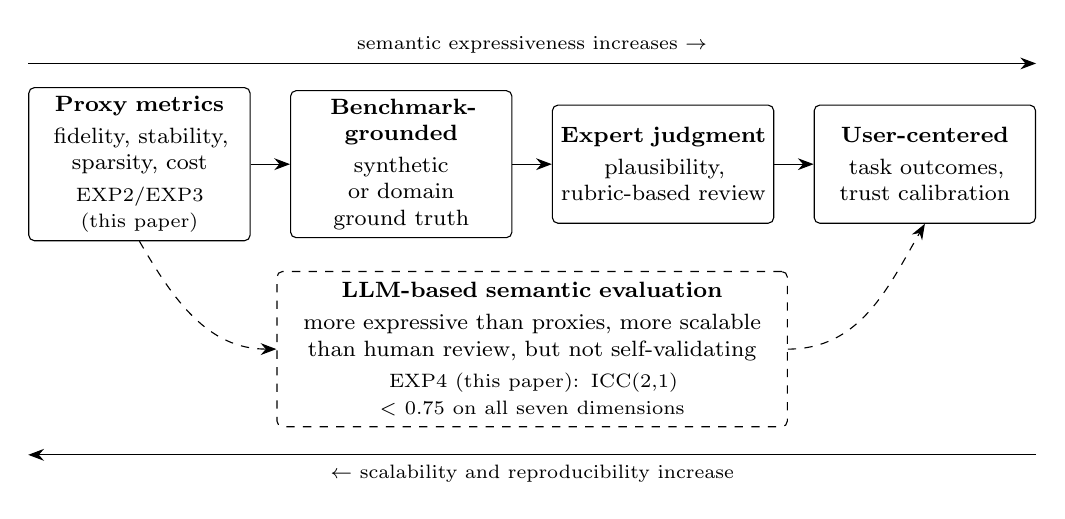
\begin{tikzpicture}[
  font=\footnotesize,
  stage/.style={draw, rounded corners=2pt, align=center,
    minimum height=1.5cm, text width=2.6cm, inner sep=3pt},
  bridge/.style={draw, dashed, rounded corners=2pt, align=center,
    text width=6.2cm, inner sep=4pt},
  >={Stealth[length=2mm]}]
\node[stage] (proxy) {\textbf{Proxy metrics}\\[2pt]
  fidelity, stability,\\ sparsity, cost\\[2pt]
  {\scriptsize EXP2/EXP3 (this paper)}};
\node[stage, right=0.5cm of proxy] (bench) {\textbf{Benchmark-grounded}\\[2pt]
  synthetic or domain\\ ground truth};
\node[stage, right=0.5cm of bench] (expert) {\textbf{Expert judgment}\\[2pt]
  plausibility,\\ rubric-based review};
\node[stage, right=0.5cm of expert] (user) {\textbf{User-centered}\\[2pt]
  task outcomes,\\ trust calibration};
\draw[->] (proxy) -- (bench);
\draw[->] (bench) -- (expert);
\draw[->] (expert) -- (user);
\node[bridge] (llm) at ($(bench.south)!0.5!(expert.south) + (0,-1.5)$)
  {\textbf{LLM-based semantic evaluation}\\[2pt]
  more expressive than proxies, more scalable than human review,
  but not self-validating\\[2pt]
  {\scriptsize EXP4 (this paper): ICC(2,1) $<$ 0.75 on all seven dimensions}};
\draw[dashed, ->] (proxy.south) to[out=-60, in=180] (llm.west);
\draw[dashed, ->] (llm.east) to[out=0, in=-120] (user.south);
\draw[->] ($(proxy.north west)+(0,0.3)$) -- ($(user.east |- proxy.north)+(0,0.3)$)
  node[midway, above] {\scriptsize semantic expressiveness increases $\rightarrow$};
\draw[->] ($(user.east |- llm.south)+(0,-0.35)$) -- ($(proxy.west |- llm.south)+(0,-0.35)$)
  node[midway, below] {\scriptsize $\leftarrow$ scalability and reproducibility increase};
\end{tikzpicture}
\caption{Evaluation continuum for post-hoc XAI, with representative metric
families mapped to each evidence layer. LLM-based semantic evaluation
occupies an intermediate position between proxy metrics and human
review; the EXP4 reliability result (Section~\ref{sec:synthesis})
shows it is not yet self-validating.}
\label{fig:continuum}
\end{figure}

Figure~\ref{fig:continuum} summarizes the evaluation continuum. Benchmark
evidence can support comparative technical claims. Semantic evaluator
outputs can support exploratory interpretation until calibrated. Human
agreement evidence can then convert those semantic constructs into
confirmatory claims.

% -----------------------------------------------------------------------
\section{Empirical Benchmark: LIME versus SHAP}
\label{sec:empirical}
% -----------------------------------------------------------------------

Section~\ref{sec:synthesis} established that proxy metrics dominate the
current evidence base while human-grounded constructs remain underspecified.
The present section fills the proxy layer with a controlled, paired
comparison of LIME and SHAP---the two most widely deployed
model-agnostic post-hoc explainers for tabular data. The study is designed
to produce auditable, scope-bounded evidence on quality-cost trade-offs
under controlled conditions, directly instantiating the ``proxy and
robustness'' cell of the layered evaluation architecture.

\subsection{Research Questions and Hypotheses}
\label{sec:rqs}

We address four directional questions:
\begin{enumerate}[leftmargin=*]
\item \textbf{RQ1 (Robustness):} Is SHAP more stable than LIME under
input perturbation?
\item \textbf{RQ2 (Parsimony):} Is LIME sparser than SHAP?
\item \textbf{RQ3 (Efficiency):} Is LIME computationally cheaper than
SHAP?
\item \textbf{RQ4 (Faithfulness):} Does SHAP provide stronger
faithfulness and fidelity signals than LIME?
\end{enumerate}

Corresponding directional hypotheses are:
\begin{enumerate}[leftmargin=*]
\item $H_1: S_{\mathrm{SHAP}} > S_{\mathrm{LIME}}$ (stability).
\item $H_2: P_{\mathrm{LIME}} > P_{\mathrm{SHAP}}$ (sparsity, measured as active-feature ratio).
\item $H_3: C_{\mathrm{LIME}} < C_{\mathrm{SHAP}}$ (cost).
\item $H_4: F_{\mathrm{SHAP}} > F_{\mathrm{LIME}}$ (fidelity/faithfulness).
\end{enumerate}

\subsection{Experimental Design and Analysis Units}
\label{sec:design}

The benchmark is instantiated from a robustness cohort with factors:
\begin{itemize}[leftmargin=*]
\item model family $g \in \{\mathrm{logreg}, \mathrm{rf}, \mathrm{xgb},
\mathrm{svm}, \mathrm{mlp}\}$,
\item explainer $k \in \{\mathrm{LIME}, \mathrm{SHAP}\}$,
\item seed $s \in \{42, 123, 456, 789, 999\}$,
\item sampling intensity $N \in \{50, 100, 200\}$ per TP/TN/FP/FN stratum.
\end{itemize}

This yields $5 \times 2 \times 5 \times 3 = 150$ planned runs, all of
which are artifact-qualified (75 LIME, 75 SHAP), forming 75 matched
SHAP-LIME cells on identical $(g, s, N)$ coordinates for paired inference.

To avoid pseudoreplication, we use a hierarchical analysis structure:
\begin{enumerate}[leftmargin=*]
\item \textbf{Instance level:} per-case metric values.
\item \textbf{Run level:} mean metric per configuration.
\item \textbf{Matched-cell level:} paired SHAP-LIME run means on shared
$(g, s, N)$ cells (primary inferential unit).
\end{enumerate}

\subsection{Data, Preprocessing, and Model Controls}
\label{sec:data}

All experiments use the UCI Adult dataset \citep{kohavi1996scaling} with
a stratified split and deterministic seeds. The preprocessing pipeline
follows train-only fitting with numeric scaling (\texttt{StandardScaler})
and categorical one-hot encoding (\texttt{OneHotEncoder};
unknowns ignored). A fixed set of pre-trained black-box models is shared across all
explainer runs to isolate explainer effects: random forest \citep{breiman2001random} and
gradient-boosted trees \citep{chen2016xgboost}, alongside logistic
regression, SVM, and MLP families. Evaluation instances are sampled by
error quadrants (TP, TN, FP, FN) via stratified sampling. Realized
instance counts range from 27 to 800 (median 400).

\subsection{Explainer Protocol}
\label{sec:explainer_protocol}

Both explainers consume the same transformed feature space and target the
positive class probability:
\begin{itemize}[leftmargin=*]
\item \textbf{SHAP:} TreeExplainer for tree models, KernelExplainer for
non-tree models, with background subsampling ($n=50$).
\item \textbf{LIME:} tabular local surrogate with
\texttt{num\_features=10}, effective \texttt{num\_samples=1000}, and
\texttt{kernel\_width=3.0}.
\end{itemize}

\subsection{Metric Operationalization}
\label{sec:metrics}

Primary metrics are computed per instance and aggregated per run:
\begin{enumerate}[leftmargin=*]
\item \textbf{Stability} $S$: mean pairwise cosine similarity of
attribution vectors under Gaussian perturbations ($T=15$, $\sigma=0.1$):
\[
S = \frac{2}{T(T-1)}\sum_{a<b}\cos\!\left(e^{(a)},e^{(b)}\right).
\]
\item \textbf{Sparsity} $P$: active-feature ratio above threshold
$\tau = 10^{-4}$ (lower active ratio indicates sparser explanations).
\item \textbf{Fidelity} $F$: faithfulness correlation between attribution
magnitude and prediction drop under feature masking.
\item \textbf{Faithfulness Gap} $\Delta_k$: absolute prediction change
after masking the top-$k$ features ($k=5$):
\[
\Delta_k = \left|f(x) - f(x_{\mathrm{mask\text{-}top\text{-}k}})\right|.
\]
\item \textbf{Cost} $C$: per-instance wall-clock explanation time (ms).
\end{enumerate}

\paragraph{Sparsity operationalization note.}
LIME's active-feature count is governed by the \texttt{num\_features=10} hyperparameter, which acts as a hard ceiling on the number of non-zero attributions returned. This means LIME sparsity is a \emph{hyperparameter constraint}, not an emergent property of the explanation model. The active-feature ratio metric therefore measures whether LIME, \emph{as configured}, returns fewer significant features than SHAP; it does not test whether LIME is intrinsically sparser under unconstrained settings. Readers comparing parsimony results across studies should verify that equivalent \texttt{num\_features} bounds are applied, since the direction and magnitude of the SHAP–LIME parsimony gap will change with different settings.

\subsection{Inferential Protocol}
\label{sec:inference}

The statistical plan follows established comparative-ML practice
\citep{demsar2006statistical}:
\begin{enumerate}[leftmargin=*]
\item primary test: two-sided paired Wilcoxon signed-rank on matched
SHAP-LIME cells for each metric \citep{wilcoxon1945individual},
\item effect size: paired $d_z$ for magnitude reporting
\citep{lakens2013calculating},
\item multiplicity control: Holm-Bonferroni over the five primary metrics
\citep{holm1979simple}.
\end{enumerate}

All inferential claims are restricted to artifact-qualified runs:
parseable, non-empty results with explicit matched pairing. No semantic
endpoint enters the confirmatory analysis reported here.

\subsection{Reproducibility Contract}
\label{sec:reproducibility}

The protocol is fully configuration-driven (YAML with seeded execution),
with per-run \texttt{results.json} artifacts, explicit exclusion of
malformed or empty runs, and no synthetic imputation. This provides a
deterministic audit trail from configuration to manuscript-level claim.

\subsection{Results}
\label{sec:results}

Results are reported from the artifact-qualified robustness cohort. The
analysis covers 150 analyzable runs (75 LIME, 75 SHAP) forming 75 paired
cells with identical $(\mathrm{model}, \mathrm{seed}, N)$. Matched
coverage spans all five model families ($\mathrm{xgb}=15$,
$\mathrm{logreg}=15$, $\mathrm{rf}=15$, $\mathrm{mlp}=15$,
$\mathrm{svm}=15$) and all sampling intensities with near-balanced counts.

\subsubsection*{Multi-Method Context (Friedman)}

As pre-analysis context, we ran a Friedman test across all four methods
in EXP2 (SHAP, LIME, Anchors \citep{ribeiro2018anchors}, DiCE
\citep{mothilal2020dice}) on $n=75$ run means per method, treating
$(g, s, N)$ combinations as blocks. The full EXP2 cohort covers all four
methods; the paired inference below is restricted to the LIME-SHAP matched
subset for confirmatory claims. Table~\ref{tab:friedman}
shows highly significant systematic differences in both fidelity and
stability (Kendall's $W > 0.90$ in both cases), establishing that the
four-method field is not exchangeable.

\begin{table}[t]
\centering
\caption{Friedman omnibus test across four methods (EXP2, $n=75$ blocks,
$k=4$). $W$ = Kendall's concordance coefficient.}
\label{tab:friedman}
\begin{tabular}{lrrl}
\toprule
Metric    & $\chi^2$ (df\,=\,3) & $p$-value             & $W$   \\
\midrule
Fidelity  & 42.12               & $1.51\times10^{-8}$  & 0.936 \\
Stability & 40.68               & $2.29\times10^{-8}$  & 0.904 \\
\bottomrule
\end{tabular}
\end{table}

Method mean values and average ranks are shown in
Table~\ref{tab:method_ranks}. Nemenyi post-hoc testing
($\mathrm{CD}=1.211$, $\alpha=0.05$) confirms that SHAP significantly
outperforms Anchors and DiCE in fidelity (rank gaps $2.2$ and $2.8$), and
significantly outperforms LIME and Anchors in stability (rank gaps
$2.4$ and $2.6$). The SHAP--DiCE stability rank gap ($1.0$) falls below
the CD threshold (Nemenyi $p = 0.15$), consistent with the comparative
run-to-run consistency of DiCE's counterfactual outputs; SHAP's stability
advantage over DiCE is therefore descriptive rather than confirmed at the
omnibus level. The SHAP-LIME omnibus fidelity rank gap equals
exactly 1.0---marginally below the CD threshold---but the directional
paired Wilcoxon below demonstrates significance when power is concentrated
on this specific two-method comparison.

\begin{table}[t]
\centering
\caption{Mean metric values by method from EXP2 ($n=75$ runs each) with
Nemenyi average ranks. CD\,=\,1.211; pairs with rank gap\,$>$\,CD are
significant at $\alpha=0.05$.}
\label{tab:method_ranks}
\begin{tabular}{lcccc}
\toprule
          & SHAP  & LIME  & Anchors & DiCE  \\
\midrule
Fidelity (mean)   & 0.808 & 0.560 & 0.389   & 0.170 \\
Stability (mean)  & 0.732 & 0.014 & 0.043   & 0.361 \\
\midrule
Fidelity rank     & 1.0   & 2.0   & 3.2     & 3.8   \\
Stability rank    & 1.0   & 3.4   & 3.6     & 2.0   \\
\bottomrule
\end{tabular}
\end{table}

\subsubsection*{Primary Paired Inference}

Table~\ref{tab:paired_main} summarizes paired run-level outcomes on the
75 matched cells. All five primary endpoints remain significant under
Holm-adjusted testing.

\begin{table}[t]
\centering
\caption{Matched SHAP-versus-LIME paired results ($n=75$ cells). For all
metrics, $\Delta = $ SHAP $-$ LIME. Sparsity is measured as
active-feature ratio; larger values indicate denser explanations.}
\label{tab:paired_main}
\begin{tabular}{lrrrrr}
\toprule
Metric & LIME Mean & SHAP Mean & $\Delta$ & $p_{\mathrm{Holm}}$ & $d_z$ \\
\midrule
Stability & 0.014 & 0.732 & +0.718 & $2.6\times10^{-13}$ & 3.00 \\
Sparsity (active ratio) & 0.085 & 0.226 & +0.142 & $2.6\times10^{-13}$ & 0.84 \\
Fidelity & 0.560 & 0.808 & +0.248 & $2.6\times10^{-13}$ & 4.82 \\
Faithfulness Gap & 0.334 & 0.380 & +0.045 & $2.6\times10^{-13}$ & 2.63 \\
Cost (ms) & 3660.7 & 11708.3 & +8047.6 & $1.2\times10^{-10}$ & 0.45 \\
\bottomrule
\end{tabular}
\end{table}

The stability effect is the largest practical separation in the study.
Median paired stability difference is $+0.866$ in favor of SHAP, and the
direction is consistent in all 75 matched cells. This indicates that
LIME's local surrogate sampling introduces substantial run-to-run
volatility under perturbation, whereas SHAP is comparatively invariant.

For sparsity, the sign is also consistent in all 75 matched cells, but
interpretation requires care: the metric here is active-feature ratio.
SHAP's larger value means denser explanations; LIME is therefore
systematically sparser and easier to compress for user-facing narratives.

Fidelity favors SHAP in all 75 matched cells, with a mean paired
difference of $+0.248$ and a very large effect size ($d_z = 4.82$).
Faithfulness gap also favors SHAP in 74 of 75 matched cells, with a mean
paired difference of $+0.045$ and a large effect size ($d_z = 2.63$).
These results indicate not only statistical separation but practically
meaningful quality gains under this protocol.
Figure~\ref{fig:quality_endpoints} visualizes the paired mean separations
for the four quality-oriented endpoints.

\begin{figure}[t]
\centering
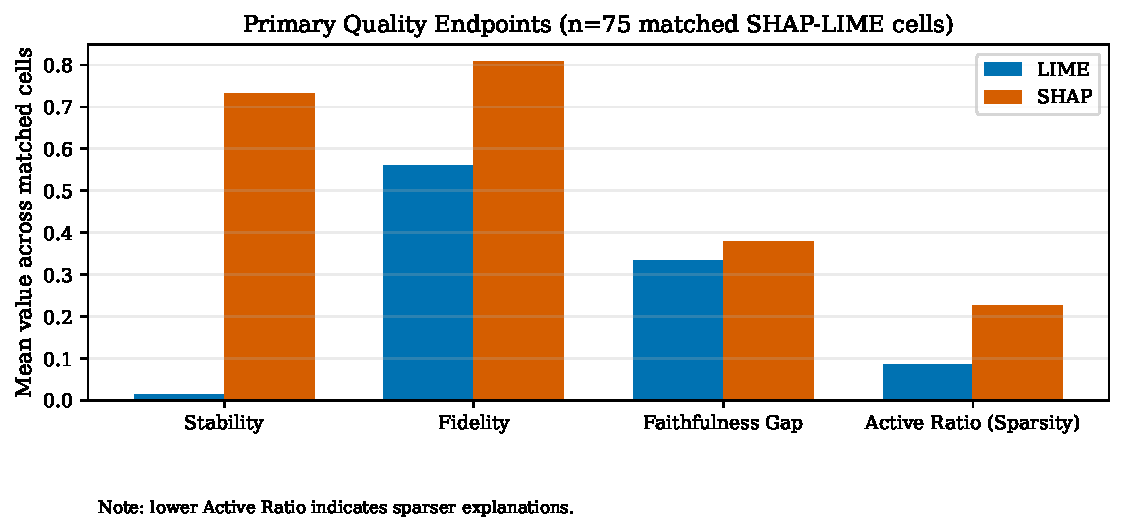
\includegraphics[width=0.95\linewidth]{figures/fig_b1_quality_endpoints.pdf}
\caption{Paired mean comparison across quality-oriented primary endpoints
($n=75$ matched SHAP-LIME cells). Active ratio is reported directly;
lower values imply sparser explanations.}
\label{fig:quality_endpoints}
\end{figure}

\subsubsection*{Reproducibility Probe}

To characterize measurement stability under seed variation, we computed
the coefficient of variation (CV\,=\,SD/mean) across the five seeds for
each $(N, \mathrm{model})$ stratum and report the stratum-median CV in
Table~\ref{tab:cv_reproducibility}. SHAP yields highly reproducible
fidelity and stability readings ($\mathrm{CV}<1\%$). LIME fidelity is
acceptable ($\mathrm{CV}=2.6\%$), whereas LIME stability is structurally
irreproducible ($\mathrm{CV}=86.2\%$). This is not a measurement artifact:
when the mean cosine similarity is $\approx 0.014$, any nonzero variation
produces an extreme relative deviation. The CV probe confirms that LIME
stability is geometrically unstable---not merely noisy.

\begin{table}[t]
\centering
\caption{Median coefficient of variation (CV\,=\,SD/mean) across seeds
per $(N, \mathrm{model})$ stratum for the two primary quality endpoints.}
\label{tab:cv_reproducibility}
\begin{tabular}{lcc}
\toprule
Method -- Metric    & Median CV & Reproducible? \\
\midrule
SHAP -- Fidelity    & 0.8\%     & Yes \\
SHAP -- Stability   & 0.7\%     & Yes \\
LIME -- Fidelity    & 2.6\%     & Yes \\
LIME -- Stability   & 86.2\%    & No  \\
\bottomrule
\end{tabular}
\end{table}

\subsubsection*{Runtime Distribution and Heterogeneity}

The cost signal is significant but strongly heterogeneous. SHAP is slower
in 59 of 75 matched cells. Matched-cell median cost is 684.1 ms for SHAP
versus 65.7 ms for LIME, corresponding to a median SHAP/LIME cost ratio
of approximately $5.3\times$. Means are more separated (11,708.3 ms vs.\
3,660.7 ms) because the SHAP distribution is heavy-tailed: the 90th and
95th percentile latencies are approximately 51,456 ms and 67,066 ms,
respectively, compared with 12,825 ms and 13,192 ms for LIME. This tail
behavior is concentrated in kernel-SHAP contexts, especially SVM.
Figure~\ref{fig:runtime_heterogeneity} shows both the overall log-scale
runtime distribution and model-level median heterogeneity.

Heterogeneity analysis by model family shows that quality ordering
(stability, sparsity-direction, fidelity, faithfulness gap) is robust,
while cost ranking is model-dependent. SHAP is faster in all 15 XGBoost
matched cells and in one SVM cell, whereas LogReg, RF, and MLP are
uniformly SHAP-slower. Therefore, ``LIME is faster'' is a majority
statement in this cohort but is not universally true across model classes.

\begin{figure}[t]
\centering
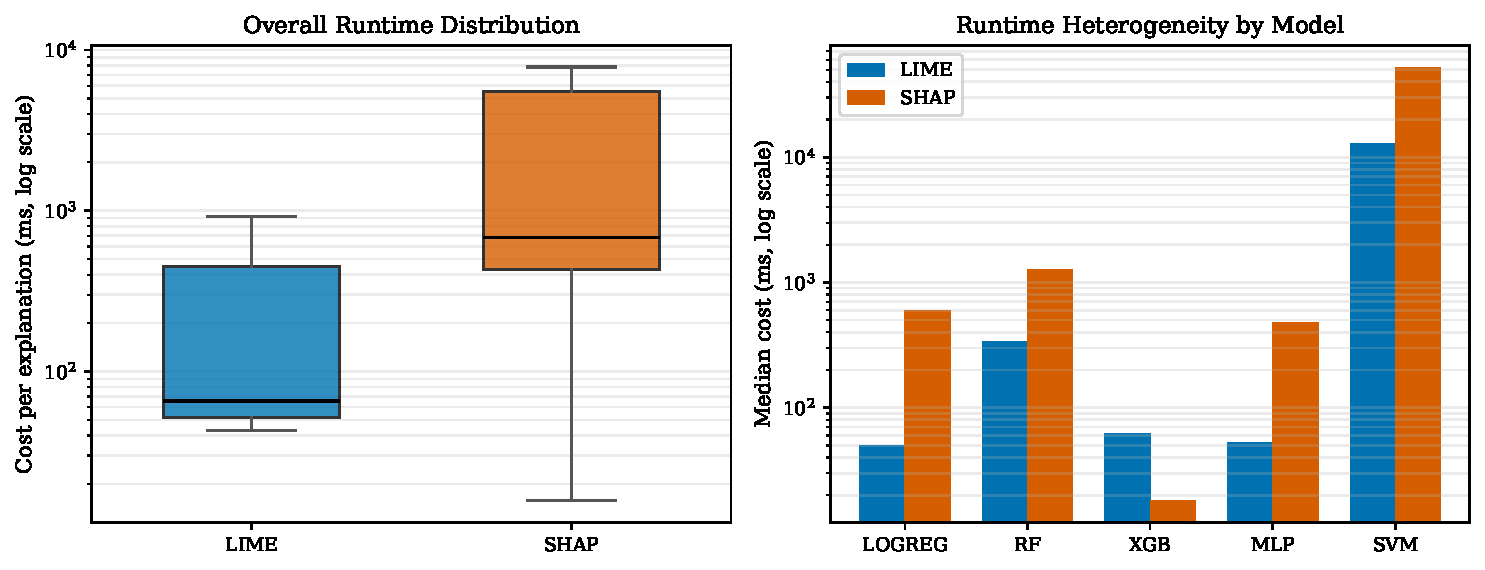
\includegraphics[width=0.98\linewidth]{figures/fig_b2_runtime_heterogeneity.pdf}
\caption{Runtime behavior under matched-cell pairing ($n=75$). Left:
overall cost distribution by method (log scale). Right: model-level
median cost (log scale), showing the XGBoost exception where SHAP is
faster while other families are SHAP-slower.}
\label{fig:runtime_heterogeneity}
\end{figure}

\subsubsection*{Synthesis of Trade-offs}

The empirical frontier is clear: SHAP delivers higher reliability and
faithfulness at substantially higher expected runtime, while LIME delivers
lower latency and stronger compression at the cost of robustness. The
results therefore support objective-driven selection rather than global
method supremacy. For assurance-critical analysis, SHAP's quality margin
is large and consistent. For interaction-critical systems, LIME's runtime
profile remains operationally attractive.

\subsection{External Validation: Cross-Dataset Replication (EXP3)}
\label{sec:exp3}

To address the single-dataset limitation, we ran a cross-dataset
validation study (EXP3) comparing SHAP, LIME, and Anchors
\citep{ribeiro2018anchors} on two additional binary classification
datasets: Breast Cancer Wisconsin \citep{dua2019uci} ($n=569$, 30
continuous features) and German Credit \citep{dua2019uci} ($n=1{,}000$,
20 mixed features). Both used random forest and XGBoost models across
three random seeds each, yielding 12 paired dataset--model--seed
comparisons per method pair.

\textbf{Fidelity ordering (SHAP vs.\ Anchors).}
SHAP outperforms Anchors in fidelity in all 12 paired combinations
(Table~\ref{tab:exp3_fidelity}, Figure~\ref{fig:exp3_fidelity}), with
mean gaps ranging from $+0.26$ (German Credit, RF) to $+0.51$ (Breast
Cancer, RF). This replicates the EXP2 fidelity direction across genuinely
different feature spaces, dimensionalities, and class distributions.

\textbf{LIME cross-dataset extension.}
Table~\ref{tab:exp3_lime} reports LIME fidelity and stability on the same
datasets. Two findings are noteworthy. First, SHAP $>$ LIME fidelity holds
consistently on German Credit (gaps $+0.23$--$+0.24$ for RF, $+0.24$--$+0.25$
for XGB), replicating the EXP2 direction. On Breast Cancer the fidelity gap
narrows substantially: SHAP leads LIME by only $+0.07$ (RF) and $+0.06$
(XGB), compared to $+0.27$ (RF) and $+0.21$ (XGB) in the corresponding
model strata on Adult. Second, and more critically, LIME
\emph{stability} on these datasets ($0.85$--$0.93$) is an order of magnitude
higher than on Adult ($0.014$). This reveals that the near-zero stability
observed in EXP2 is not a fixed structural property of LIME: it is strongly
modulated by feature-space characteristics. The Adult dataset's 103-dimensional
one-hot-encoded space appears to be the primary driver of instability; in
lower-dimensional spaces with more continuous features, LIME produces
substantially more consistent explanations.

\begin{table}[t]
\centering
\caption{EXP3 external validation: mean fidelity (3-seed average) for
SHAP vs.\ Anchors across two additional datasets. SHAP $>$ Anchors in all
12 paired combinations.}
\label{tab:exp3_fidelity}
\begin{tabular}{llcc}
\toprule
Dataset        & Model & SHAP  & Anchors \\
\midrule
Breast Cancer  & RF    & 0.779 & 0.265   \\
Breast Cancer  & XGB   & 0.607 & 0.208   \\
German Credit  & RF    & 0.714 & 0.351   \\
German Credit  & XGB   & 0.711 & 0.451   \\
\bottomrule
\end{tabular}
\end{table}

\begin{table}[t]
\centering
\caption{EXP3 LIME extension: mean fidelity and stability (3-seed average)
for LIME on the two cross-dataset cohorts.
Stability = mean pairwise cosine similarity under $T=15$ Gaussian
perturbations ($\sigma=0.1$); same protocol as EXP2.
For comparison, LIME on Adult (EXP2) in the matched model strata:
fidelity $0.457$ (RF) and $0.553$ (XGB); stability $\approx 0.01$--$0.02$
across all model families.}
\label{tab:exp3_lime}
\begin{tabular}{llcccc}
\toprule
Dataset        & Model & Fidelity & Stability & Sparsity & Cost (ms) \\
\midrule
Breast Cancer  & RF    & 0.713    & 0.922     & 0.331    & 12.3 \\
Breast Cancer  & XGB   & 0.543    & 0.927     & 0.331    & 7.5  \\
German Credit  & RF    & 0.483    & 0.854     & 0.163    & 21.1 \\
German Credit  & XGB   & 0.468    & 0.748     & 0.163    & 10.2 \\
\bottomrule
\end{tabular}
\end{table}

\textbf{Scope limitation.} SHAP stability on the cross-dataset cohorts was
not instrumented in EXP3; a direct SHAP--LIME stability comparison on Breast
Cancer and German Credit remains pending. The finding that LIME stability
varies dramatically with feature-space dimensionality and encoding density
should be taken as a moderation hypothesis requiring further confirmation
across a broader set of datasets and preprocessing schemes.

\begin{figure}[t]
\centering
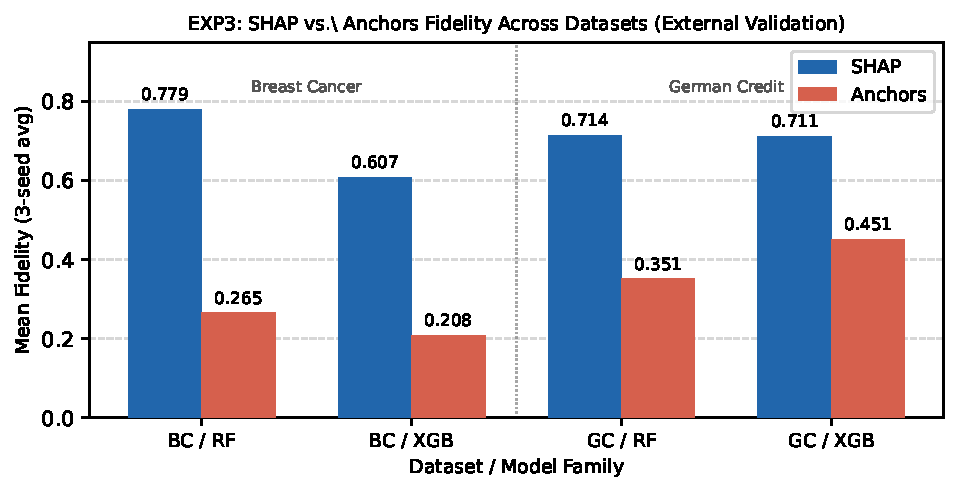
\includegraphics[width=0.95\linewidth]{figures/fig_exp3_fidelity.pdf}
\caption{EXP3 external validation: mean fidelity (3-seed average) for
SHAP vs.\ Anchors across four dataset-model combinations. SHAP exceeds
Anchors in all 12 paired (dataset $\times$ model $\times$ seed)
combinations. BC\,=\,Breast Cancer; GC\,=\,German Credit.}
\label{fig:exp3_fidelity}
\end{figure}

% -----------------------------------------------------------------------
\section{Practical Recommendations}
\label{sec:recommendations}
% -----------------------------------------------------------------------

Based on the taxonomy (Section~\ref{sec:taxonomy}), the gap analysis
(Section~\ref{sec:synthesis}), and the empirical findings
(Section~\ref{sec:empirical}), we propose the \textbf{Hybrid Deployment
Pattern}:

\begin{enumerate}[leftmargin=*]
\item \textbf{Tier 1: Real-Time / End-User}
\begin{itemize}[leftmargin=*]
\item \textbf{Primary selection criterion: model architecture.}
  For \emph{tree-based models} (e.g., XGBoost, LightGBM, Random Forest),
  use \textbf{SHAP} with \texttt{TreeExplainer}.  The algorithm computes
  exact Shapley values in $O(TLD)$ time (trees~$\times$ leaves~$\times$
  depth), which in this cohort consistently undercuts LIME's perturbation
  sampling loop even at the lowest sample budgets.  The fidelity--latency
  trade-off that motivates Tier~1 therefore does not apply: SHAP is
  simultaneously faster \emph{and} more faithful on tree architectures.
  For \emph{non-tree or black-box models} (e.g., neural networks, opaque
  APIs), use \textbf{LIME}; lower median runtime on non-tree cells
  (53.3~ms vs.\ 694.6~ms for KernelSHAP) and a compact active-feature
  ratio give it a meaningful latency advantage where perturbation
  sampling is the only option.
\item Recommended condition: interactive settings where sub-second latency
  and compact explanations matter more than maximising fidelity, \emph{and}
  no model-aware explainer is available.
\item Evidence basis: runtime distribution in
  Figure~\ref{fig:runtime_heterogeneity}; XGBoost reversal visible as a
  structural outlier, not an anomaly.
\end{itemize}
\item \textbf{Tier 2: Auditing / Data Science (Use SHAP)}
\begin{itemize}[leftmargin=*]
\item Use when analyzing model bias, debugging model logic, or responding
to regulatory inquiries.
\item Evidence basis: consistent paired advantages in stability, fidelity,
and faithfulness gap across the matched cohort ($d_z = 3.00$, $4.82$, and
$2.63$ respectively).
\item Recommended condition: analyst-mediated or offline workflows where
second-level or minute-level latency is acceptable.
\item Note: runtime costs in this tier depend on whether SHAP operates in
tree-specific or kernel mode; plan sample budgets accordingly.
\end{itemize}
\end{enumerate}

This two-tier pattern directly reflects the layered evaluation
architecture identified in Section~\ref{sec:synthesis}: proxy and
benchmark evidence (Tier~2) can be complemented by interaction-optimised
lightweight explanations (Tier~1), each operating within its validated
scope.  Critically, the Tier~1 criterion is not a blanket method preference
but a function of model architecture: the existence of a model-aware
explainer (e.g., \texttt{TreeExplainer}) collapses the fidelity--latency
trade-off, making SHAP the dominant choice at both tiers for tree-based
deployments.  This maps directly onto the Task Context axis of the taxonomy
(Section~\ref{sec:taxonomy}): explainer selection is determined first by
architectural affordance, then by deployment constraint.

% -----------------------------------------------------------------------
\section{Validity Boundaries and Limitations}
\label{sec:validity}
% -----------------------------------------------------------------------

\subsection{Interpretation Scope of SHAP--LIME Comparisons}
\label{sec:interpretation_scope}

The SHAP--LIME differences reported here should be interpreted as
comparative performance within our benchmark protocol, not as definitive
evidence that one method is universally more correct. Recent formal
analyses show that multiple attribution families can produce
high-importance assignments to suppressor variables in
dependent-feature settings, complicating direct interpretation of
attribution magnitude as target-relevant importance
\citep{wilming2022scrutinizing,wilming2023theoretical,haufe2026formalization}.
Observed performance gaps between SHAP and LIME may therefore reflect both
methodological differences and sensitivity to data dependence structure.

We distinguish \emph{ranking claims} from \emph{validity claims}. A
ranking claim states that one explainer outperforms another on predefined
benchmark criteria in this dataset and protocol. A validity claim would
require stronger evidence that explanations satisfy a formal correctness
criterion for the intended task, potentially including controlled
ground-truth tests and explicit assumption checks
\citep{haufe2026formalization,doshivelez2017rigorous}. This paper
primarily makes ranking claims; broader validity claims remain provisional.

This framing aligns with prior findings that faithfulness-style evaluations
can be informative but are not sufficient to resolve correctness questions
in isolation \citep{jacovi2020faithfulness,adebayo2018sanity,
hooker2019benchmark,rong2022consistent}. The SHAP--LIME comparison
presented here is best read as robust comparative evidence under the
evaluated conditions, with external validity depending on how closely
downstream applications match those conditions.

\subsection{Taxonomy Scope and Single-Reviewer Limitation}

The survey employs a structured database search with documented inclusion
and exclusion criteria and a PRISMA-style screening record
(Table~\ref{tab:prisma}). It is not, however, a full systematic review:
the search used five databases rather than an exhaustive database set,
and the title/abstract screen was performed by a single reviewer. The emphasis on model-agnostic
post-hoc XAI reflects the scope of the empirical study; intrinsic
interpretability and some modality-specific traditions are covered only
insofar as they affect metric transfer. The coding pass is single-reviewer
and inherits records at varying confidence levels from the upstream matrix.
Future versions should deepen lower-confidence entries through full-text
coding or replace them with higher-confidence sources. The taxonomy
organizes construct space---not effect sizes---and does not estimate a
pooled numerical ranking across studies.

\subsection{Statistical and Construct Validity}

Confirmatory claims are restricted to the 75 fully matched SHAP-LIME
cells in the robustness cohort. All 75 LIME and 75 SHAP runs are artifact-qualified and available
for paired inference. Reported metrics are implementation-bound
rather than abstract labels; their operational definitions are anchored
in the companion repository source files for fidelity, stability,
sparsity, faithfulness, and cost. No semantic, human-utility, or
LLM-judge claim enters the confirmatory scope.

\paragraph{Axiomatic properties and metric alignment.}
SHAP satisfies four axioms---dummy, linearity, symmetry, and efficiency---that
guarantee attributions distribute the full prediction change $f(x) -
\mathbb{E}[f]$ as uniquely fair marginal contributions.
Perturbation-based fidelity metrics measure whether high-magnitude attributions
correspond to large prediction drops under feature masking.
These two perspectives are structurally compatible: both quantify how faithfully
attribution magnitudes encode feature-level causal responsibility for the model
output. SHAP's axiomatic guarantee implies that, conditional on its background
distribution assumptions, its attribution rankings are optimally aligned with
the feature-removal signal that fidelity metrics probe. This does not mean SHAP
axioms certify correctness in all deployment contexts---the axioms hold for the
model, not for any latent data-generative mechanism---but it does explain why
SHAP consistently outperforms LIME on perturbation-based fidelity without
requiring that LIME violates a formal criterion.

\subsection{Internal and External Validity}

Runtime comparisons are protocol-specific. SHAP combines TreeExplainer
for tree models and KernelExplainer for non-tree models, whereas LIME is
run with fixed local-surrogate settings (\texttt{num\_features=10},
effective \texttt{num\_samples=1000}, \texttt{kernel\_width=3.0}).
Accordingly, the reported cost gap reflects both method family and
concrete implementation pathway. External generalization is partially
supported by EXP3 (Section~\ref{sec:exp3}), which replicates SHAP's
fidelity advantage over Anchors across Breast Cancer and German Credit
datasets; SHAP-LIME comparisons and stability rankings remain bounded to
the Adult cohort and may shift under different modalities, feature
transformations, masking schemes, or hyperparameter settings.

\paragraph{LIME stability is not a convergence artifact.}
A direct test of whether the near-zero LIME stability (cosine similarity mean $\approx
0.014$, CV $= 86.2\%$) reflects insufficient perturbation samples was conducted
by varying \texttt{num\_samples} $\in \{500, 1000, 2000\}$ under otherwise
identical conditions (RF model, seed 42, $N=100$, \texttt{kernel\_width=3.0}).
Stability remained near-zero at all levels ($0.011$, $0.014$, $0.016$,
respectively), while fidelity was essentially flat ($0.452$, $0.461$, $0.459$).
Doubling or halving the sample budget neither stabilizes the explanations nor
changes the fidelity ordering. The instability is therefore structural---it
reflects inherent variability in LIME's local surrogate fitting process under
Gaussian input perturbation, not an insufficient sample count that more compute
would resolve. A companion \texttt{kernel\_width} probe ($0.25$, $0.75$, $3.0$,
$10.0$) further shows that widths below $3.0$ produce degenerate zero-weight
explanations in this 103-dimensional preprocessed space, confirming that the
reference setting is the minimum viable configuration rather than a conservative
choice (see companion repository, \path{outputs/analysis/}).

\paragraph{Feature correlation and out-of-distribution masking.}
The Adult Income dataset contains moderate inter-feature correlations that affect the validity of perturbation-based fidelity metrics. Notably, \texttt{education} and \texttt{education-num} encode the same ordinal construct ($r = 1.0$ by construction); \texttt{occupation} and \texttt{education} show moderate Cramér's $V \approx 0.34$; and \texttt{hours-per-week} correlates with \texttt{occupation} and \texttt{workclass}. When these features are independently zeroed or replaced by reference values during masking---as in our fidelity and faithfulness-gap computations---the resulting masked instances may fall outside the training distribution. Under such out-of-distribution (OOD) inputs, tree-based model outputs can be unreliable extrapolations, and the correlation structure between masked and retained features is ignored. This can cause fidelity metrics to either overestimate (if the model is insensitive to OOD inputs) or underestimate (if the model reacts to implausible feature combinations) the true attribution quality. We cannot rule out that some portion of the SHAP--LIME fidelity gap reflects differential sensitivity to OOD masking artifacts rather than solely attribution accuracy. Studies using marginal versus conditional SHAP variants, or masking schemes that preserve feature dependencies, are needed to isolate this contribution.

\subsection{Reproducibility and Operational Validity}

All reported claims are traceable to seeded YAML configurations, per-run
\texttt{results.json} artifacts, explicit exclusion of malformed or empty
runs, and inferential exports in the companion repository. Figures are
regenerated directly from the paired-cell Wilcoxon exports; no synthetic
imputation is used at any stage. Before journal submission, the exact
review snapshot should be frozen as a versioned release and archived under
a version-specific DOI.

\subsection{Future Work}

Several limitations define natural extensions:
\begin{itemize}[leftmargin=*]
\item \textbf{Dataset scope:} The primary paired benchmark focuses on the
Adult tabular dataset; EXP3 partially extends fidelity replication to
Breast Cancer and German Credit. Image, text, and graph domains remain
untested and may exhibit different trade-offs.
\item \textbf{Configuration space:} Both methods were run with default
hyperparameter settings. A dedicated kernel-width probe (four values: 0.25,
0.75, 3.0, 10.0) reveals that values below 3.0 are degenerate in the
103-dimensional preprocessed Adult feature space---all weights collapse to
zero---while $\mathtt{kernel\_width}=10.0$ yields full instance coverage
and improved stability (0.664 vs.\ near-zero) at a modest fidelity cost
(0.441 vs.\ 0.518). These results confirm that the reference setting
(3.0) is the minimum viable value in this space, not a conservative choice,
and that the LIME instability observed in EXP2 persists across kernel-width
settings rather than reflecting a calibration artifact. SHAP background-set
sensitivity and cross-model kernel-width effects remain open.
\item \textbf{Runtime heterogeneity:} The XGBoost exception shows that
``LIME is faster'' is not a universal rule and warrants tree-specific analysis.
\item \textbf{Human-centered utility:} This paper does not establish
human-grounded usefulness; validated user studies with task-outcome
measures remain future work.
\item \textbf{LLM-judge calibration:} EXP4 shows that ICC remains below
0.75 for all seven semantic dimensions; developing rubrics that achieve
calibration-grade inter-rater agreement is an open challenge.
\item \textbf{Taxonomy completeness:} The survey corpus is a working
corpus rather than an exhaustive bibliometric sample; expanding it with
systematic search protocols would strengthen the gap analysis.
\item \textbf{Causal and counterfactual endpoints:} Integration of
causal attribution methods and diverse counterfactual generation
\citep{mothilal2020dice} remains an open follow-up.
\end{itemize}

% -----------------------------------------------------------------------
\section{Code and Artifact Availability}
\label{sec:artifacts}
% -----------------------------------------------------------------------

The manuscript, experimental code, and supporting materials are available
in the public repository at
\url{https://github.com/jonnabio/xai-eval-framework}, released under the
MIT License. Artifacts needed to reproduce the empirical study include:
\begin{sloppypar}
\begin{itemize}[leftmargin=*]
\item EXP2 results: \path{experiments/exp2_scaled/results/}
\item EXP2 inferential exports: \path{outputs/analysis/exp2_stats/}
(includes \path{analysis_summary.json},
\path{wilcoxon_shap_lime_all_models.csv},
\path{paired_cells_shap_lime_all_models.csv})
\item EXP3 results: \path{experiments/exp3/results/}
\item EXP4 ICC exports: \path{outputs/analysis/exp4_llm_evaluation/}
\item analysis scripts: \path{scripts/run_exp2_statistical_analysis.py},
\path{scripts/generate_paper_b_figures.py}
\end{itemize}
\end{sloppypar}

The review corpus CSV underlying the taxonomy and gap analysis is also
available in the companion repository. Before journal submission, the
exact snapshot will be frozen as a versioned release with a DOI.

% -----------------------------------------------------------------------
\section{Conclusion}
\label{sec:conclusion}
% -----------------------------------------------------------------------

XAI evaluation is not one problem but a family of related measurement
problems. The literature has developed useful metric families for fidelity,
robustness, sparsity, and benchmark reproducibility, yet these families do
not fully capture semantic adequacy or human-centered meaning. By
organizing model-agnostic post-hoc evaluation along the axes of evaluation
target, evidence source, quality property, and task context, this paper
clarifies why metric disagreement is common and why layered evaluation is
necessary.

The main practical implication is twofold. First, benchmark metrics and
semantic evaluation should be treated as complementary rather than
competing forms of evidence. The taxonomy makes explicit where each
metric family gains strength and where it leaves blind spots. Second, the
choice between LIME and SHAP is not a matter of one being universally
better but of fit for purpose. Under the paired benchmark protocol, SHAP
is the preferred choice when stability and fidelity-oriented quality
dominate the objective, while LIME remains the pragmatic option when
latency and compactness are the primary constraints.

Our paired analysis across 75 matched robustness cells shows consistent
SHAP advantages in stability ($d_z = 3.00$), fidelity ($d_z = 4.82$),
and faithfulness gap ($d_z = 2.63$), alongside systematic LIME advantages
in sparsity and lower runtime for most model contexts. Cross-dataset
replication (EXP3) confirms SHAP's fidelity advantage over Anchors across
all 12 paired combinations on two independent datasets, strengthening the
generalizability of the fidelity ranking. These results, read through the
lens of the taxonomy, support a layered deployment architecture that
separates user-facing low-latency explanation paths from high-assurance
auditing workflows.

\acks{This work received no external funding. The study was self-funded by
the author, and the author reports no competing interests. This draft was
prepared from repository artifacts dated May 2026.}

\clearpage
\phantomsection
\pdfbookmark[1]{References}{references}
\begin{thebibliography}{99}

\bibitem[Adadi and Berrada(2018)]{adadi2018xai}
Adadi, A. and Berrada, M. (2018).
Peeking inside the black-box: A survey on explainable artificial
intelligence (XAI).
\emph{IEEE Access}, 6:52138--52160.

\bibitem[Adebayo et~al.(2018)Adebayo, Gilmer, Muelly, Goodfellow, Hardt,
and Kim]{adebayo2018sanity}
Adebayo, J., Gilmer, J., Muelly, M., Goodfellow, I., Hardt, M., and Kim, B.
(2018).
Sanity checks for saliency maps.
In \emph{Advances in Neural Information Processing Systems}, volume~31,
9525--9536.

\bibitem[Agarwal et~al.(2022)Agarwal, Ley, Krishna, Saxena, Pawelczyk,
Johnson, Puri, Zitnik, and Lakkaraju]{agarwal2022openxai}
Agarwal, C., Ley, D., Krishna, S., Saxena, E., Pawelczyk, M., Johnson, N.,
Puri, I., Zitnik, M., and Lakkaraju, H. (2022).
OpenXAI: Towards a transparent evaluation of model explanations.
In \emph{Thirty-Sixth Conference on Neural Information Processing Systems
Datasets and Benchmarks Track}.
\url{https://openreview.net/forum?id=MU2495w47rz}.

\bibitem[Agarwal et~al.(2023)Agarwal, Queen, Lakkaraju, and
Zitnik]{agarwal2023gnn_eval}
Agarwal, C., Queen, O., Lakkaraju, H., and Zitnik, M. (2023).
Evaluating explainability for graph neural networks.
\emph{Scientific Data}, 10:144.

\bibitem[Agrawal et~al.(2025)Agrawal, El~Shawi, and Ahmed]{agrawal2025xaieval}
Agrawal, K., El~Shawi, R., and Ahmed, N. (2025).
XAI-Eval: A framework for comparative evaluation of explanation methods
in healthcare.
\emph{DIGITAL HEALTH}, 11:20552076251368045.
\url{https://doi.org/10.1177/20552076251368045}.

\bibitem[Ali et~al.(2023)Ali, Abuhmed, El-Sappagh, Muhammad, Alonso-Moral,
Confalonieri, Guidotti, Del~Ser, D\'{i}az-Rodr\'{i}guez, and
Herrera]{ali2023trustworthy}
Ali, S., Abuhmed, T., El-Sappagh, S., Muhammad, K., Alonso-Moral, J.~M.,
Confalonieri, R., Guidotti, R., Del~Ser, J., D\'{i}az-Rodr\'{i}guez, N.,
and Herrera, F. (2023).
Explainable Artificial Intelligence (XAI): What we know and what is left
to attain Trustworthy Artificial Intelligence.
\emph{Information Fusion}, 99:101805.
\url{https://doi.org/10.1016/j.inffus.2023.101805}.

\bibitem[Alvarez-Melis and Jaakkola(2018)]{alvarezmelis2018robustness}
Alvarez-Melis, D. and Jaakkola, T.~S. (2018).
On the robustness of interpretability methods.
In \emph{ICML Workshop on Human Interpretability in Machine Learning
(WHI 2018)}.
\url{https://arxiv.org/abs/1806.08049}.

\bibitem[Arrieta et~al.(2020)Arrieta, D\'{i}az-Rodr\'{i}guez, Del~Ser,
et~al.]{arrieta2020xai}
Arrieta, A.~B., D\'{i}az-Rodr\'{i}guez, N., Del~Ser, J., et~al. (2020).
Explainable artificial intelligence (XAI): Concepts, taxonomies,
opportunities and challenges toward responsible AI.
\emph{Information Fusion}, 58:82--115.

\bibitem[Bansal et~al.(2021)Bansal, Wu, Vaughan, and Wallach]{bansal2021whole}
Bansal, G., Wu, T., Vaughan, J., and Wallach, H. (2021).
Does the whole exceed its parts? The effect of AI explanations on
complementary team performance.
In \emph{Proceedings of the CHI Conference on Human Factors in Computing
Systems}, 1--16.

\bibitem[Breiman(2001)]{breiman2001random}
Breiman, L. (2001).
Random forests.
\emph{Machine Learning}, 45(1):5--32.

\bibitem[Bu\c{c}inca et~al.(2020)Bu\c{c}inca, Lin, Gajos, and
Glassman]{bucinca2020proxy}
Bu\c{c}inca, Z., Lin, P., Gajos, K.~Z., and Glassman, E.~L. (2020).
Proxy tasks and subjective measures can be misleading in evaluating
explainable AI systems.
In \emph{Proceedings of the 25th International Conference on Intelligent
User Interfaces}, 454--464.

\bibitem[Burkart and Huber(2021)]{burkart2021survey}
Burkart, N. and Huber, M.~F. (2021).
A survey on the explainability of supervised machine learning.
\emph{Journal of Artificial Intelligence Research}, 70:245--317.
\url{https://doi.org/10.1613/jair.1.12228}.

\bibitem[Canha et~al.(2025)Canha, Kubler, Fr\"{a}mling, and
Fagherazzi]{canha2025benchmark}
Canha, D., Kubler, S., Fr\"{a}mling, K., and Fagherazzi, G. (2025).
A functionally-grounded benchmark framework for XAI methods: Insights
and foundations from a systematic literature review.
\emph{ACM Computing Surveys}, 57(12):1--40.
\url{https://doi.org/10.1145/3737445}.

\bibitem[Chen and Guestrin(2016)]{chen2016xgboost}
Chen, T. and Guestrin, C. (2016).
XGBoost: A scalable tree boosting system.
In \emph{Proceedings of the 22nd ACM SIGKDD International Conference on
Knowledge Discovery and Data Mining}, 785--794.

\bibitem[Covert et~al.(2020)Covert, Lundberg, and Lee]{covert2020sage}
Covert, I., Lundberg, S., and Lee, S.-I. (2020).
Understanding global feature contributions with additive importance
measures.
In \emph{Advances in Neural Information Processing Systems 33},
17212--17223.
\url{https://arxiv.org/abs/2004.00668}.

\bibitem[Dems\v{a}r(2006)]{demsar2006statistical}
Dems\v{a}r, J. (2006).
Statistical comparisons of classifiers over multiple data sets.
\emph{Journal of Machine Learning Research}, 7:1--30.

\bibitem[Doshi-Velez and Kim(2017)]{doshivelez2017rigorous}
Doshi-Velez, F. and Kim, B. (2017).
Towards a rigorous science of interpretable machine learning.
\emph{arXiv preprint arXiv:1702.08608}.
\url{https://arxiv.org/abs/1702.08608}.

\bibitem[Dua and Graff(2019)]{dua2019uci}
Dua, D. and Graff, C. (2019).
{UCI} Machine Learning Repository.
University of California, Irvine, School of Information and Computer Science.
\url{http://archive.ics.uci.edu/ml}.

\bibitem[Fok and Weld(2023)]{fok2023verifiability}
Fok, R. and Weld, D.~S. (2023).
In search of verifiability: Explanations rarely enable complementary
performance in AI-advised decision making.
\emph{AI Magazine}, 45(3):317--332.

\bibitem[Gu et~al.(2024)Gu, Jiang, Shi, Tan, Zhai, Xu, Li, Shen, Ma,
Liu, Wang, Zhang, Wang, Gao, Ni, and Guo]{gu2024llmjudge}
Gu, J., Jiang, X., Shi, Z., Tan, H., Zhai, X., Xu, C., Li, W., Shen, Y.,
Ma, S., Liu, H., Wang, S., Zhang, K., Wang, Y., Gao, W., Ni, L., and
Guo, J. (2024).
A survey on LLM-as-a-Judge.
\emph{arXiv preprint arXiv:2411.15594}.
\url{https://doi.org/10.48550/arXiv.2411.15594}.

\bibitem[Guidotti et~al.(2018)Guidotti, Monreale, Ruggieri, Turini,
Giannotti, and Pedreschi]{guidotti2018survey}
Guidotti, R., Monreale, A., Ruggieri, S., Turini, F., Giannotti, F.,
and Pedreschi, D. (2018).
A survey of methods for explaining black box models.
\emph{ACM Computing Surveys}, 51(5):93:1--93:42.
\url{https://doi.org/10.1145/3236009}.

\bibitem[Hase and Bansal(2020)]{hase2020evaluating}
Hase, P. and Bansal, M. (2020).
Evaluating explainable {AI}: Which algorithmic explanations help users
predict model behavior?
In \emph{Proceedings of the 58th Annual Meeting of the Association for
Computational Linguistics}, 5540--5552.
\url{https://doi.org/10.18653/v1/2020.acl-main.491}.

\bibitem[Haufe et~al.(2026)Haufe, Wilming, Clark, Zhumagambetov, Boubekki,
Martin, and Panknin]{haufe2026formalization}
Haufe, S., Wilming, R., Clark, B., Zhumagambetov, R., Boubekki, A.,
Martin, J., and Panknin, D. (2026).
Explainable {AI} needs formalization.
\emph{npj Artificial Intelligence}, 2:42.
\url{https://doi.org/10.1038/s44387-026-00095-1}.

\bibitem[Hedstrom et~al.(2023)Hedstrom, Weber, Bareeva, Krakowczyk,
Motzkus, Samek, Lapuschkin, and Hohne]{hedstrom2023quantus}
Hedstrom, A., Weber, L., Bareeva, D., Krakowczyk, D., Motzkus, F.,
Samek, W., Lapuschkin, S., and Hohne, M.~M.-C. (2023).
Quantus: An explainable AI toolkit for responsible evaluation of neural
network explanations and beyond.
\emph{Journal of Machine Learning Research}, 24:1--11.

\bibitem[Holm(1979)]{holm1979simple}
Holm, S. (1979).
A simple sequentially rejective multiple test procedure.
\emph{Scandinavian Journal of Statistics}, 6(2):65--70.

\bibitem[Hooker et~al.(2019)Hooker, Erhan, Kindermans, and
Kim]{hooker2019benchmark}
Hooker, S., Erhan, D., Kindermans, P.-J., and Kim, B. (2019).
A benchmark for interpretability methods in deep neural networks.
In \emph{Advances in Neural Information Processing Systems}, volume~32,
9737--9748.

\bibitem[Jacovi and Goldberg(2020)]{jacovi2020faithfulness}
Jacovi, A. and Goldberg, Y. (2020).
Towards faithfully interpretable {NLP} systems: How should we define and
evaluate faithfulness?
In \emph{Proceedings of the 58th Annual Meeting of the Association for
Computational Linguistics}, 4198--4205.

\bibitem[Kadir et~al.(2023)Kadir, Mosavi, and Sonntag]{kadir2023metrics}
Kadir, M.~A., Mosavi, A., and Sonntag, D. (2023).
Evaluation metrics for XAI: A review, taxonomy, and practical applications.
In \emph{Proceedings of the IEEE 27th International Conference on
Intelligent Engineering Systems}, 111--124.

\bibitem[Kaur et~al.(2020)Kaur, Nori, Jenkins, Caruana, Wallach, and
Vaughan]{kaur2020interpreting}
Kaur, H., Nori, H., Jenkins, S., Caruana, R., Wallach, H., and
Vaughan, J.~W. (2020).
Interpreting interpretability: Understanding data scientists' use of
interpretability tools for machine learning.
In \emph{Proceedings of the 2020 {CHI} Conference on Human Factors in
Computing Systems}, 1--14.
\url{https://doi.org/10.1145/3313831.3376219}.

\bibitem[Kohavi(1996)]{kohavi1996scaling}
Kohavi, R. (1996).
Scaling up the accuracy of Naive-Bayes classifiers: A decision-tree hybrid.
In \emph{Proceedings of the Second International Conference on Knowledge
Discovery and Data Mining}, 202--207.

\bibitem[Koo and Li(2016)]{koo2016guideline}
Koo, T.~K. and Li, M.~Y. (2016).
A guideline of selecting and reporting intraclass correlation coefficients
for reliability research.
\emph{Journal of Chiropractic Medicine}, 15(2):155--163.
\url{https://doi.org/10.1016/j.jcm.2016.02.012}.

\bibitem[Kumar et~al.(2020)Kumar, Venkatasubramanian, Scheidegger, and
Friedler]{kumar2020problems}
Kumar, I.~E., Venkatasubramanian, S., Scheidegger, C., and
Friedler, S.~A. (2020).
Problems with {Shapley}-value-based explanations as feature importance
measures.
In \emph{Proceedings of the 37th International Conference on Machine
Learning}, 5491--5500.
\url{https://arxiv.org/abs/2002.11097}.

\bibitem[Lakens(2013)]{lakens2013calculating}
Lakens, D. (2013).
Calculating and reporting effect sizes to facilitate cumulative science:
A practical primer for $t$-tests and ANOVAs.
\emph{Frontiers in Psychology}, 4:863.

\bibitem[Lipton(2018)]{lipton2018mythos}
Lipton, Z.~C. (2018).
The mythos of model interpretability.
\emph{Queue}, 16(3):31--57.
\url{https://doi.org/10.1145/3236386.3241340}.

\bibitem[Longo et~al.(2024)Longo, Brcic, Cabitza, Choi, Confalonieri,
Del~Ser, Guidotti, Hayashi, Herrera, Holzinger, Jiang, Khosravi, Lecue,
Malgieri, P\'{a}ez, Samek, Schneider, Speith, and
Stumpf]{longo2024manifesto}
Longo, L., Brcic, M., Cabitza, F., Choi, J., Confalonieri, R., Del~Ser, J.,
Guidotti, R., Hayashi, Y., Herrera, F., Holzinger, A., Jiang, R.,
Khosravi, H., Lecue, F., Malgieri, G., P\'{a}ez, A., Samek, W.,
Schneider, J., Speith, T., and Stumpf, S. (2024).
Explainable artificial intelligence (XAI) 2.0: A manifesto of open
challenges and interdisciplinary research directions.
\emph{Information Fusion}, 106:102301.
\url{https://doi.org/10.1016/j.inffus.2024.102301}.

\bibitem[Lundberg and Lee(2017)]{lundberg2017unified}
Lundberg, S.~M. and Lee, S.-I. (2017).
A unified approach to interpreting model predictions.
In \emph{Advances in Neural Information Processing Systems}, 4765--4774.

\bibitem[Mohseni et~al.(2021)Mohseni, Zarei, and Ragan]{mohseni2021survey}
Mohseni, S., Zarei, N., and Ragan, E.~D. (2021).
A multidisciplinary survey and framework for design and evaluation of
explainable {AI} systems.
\emph{{ACM} Transactions on Interactive Intelligent Systems},
11(3--4):1--45.
\url{https://doi.org/10.1145/3387166}.

\bibitem[Mothilal et~al.(2020)Mothilal, Sharma, and Tan]{mothilal2020dice}
Mothilal, R.~K., Sharma, A., and Tan, C. (2020).
Explaining machine learning classifiers through diverse counterfactual
explanations.
In \emph{Proceedings of the 2020 Conference on Fairness, Accountability,
and Transparency}, 607--617.

\bibitem[Nauta et~al.(2023)Nauta, Trienes, Pathak, Nguyen, Peters,
Schmitt, Schlötterer, van Keulen, and Seifert]{nauta2023anecdotal}
Nauta, M., Trienes, J., Pathak, S., Nguyen, E., Peters, M., Schmitt, Y.,
Schl\"{o}tterer, J., van Keulen, M., and Seifert, C. (2023).
From anecdotal evidence to quantitative evaluation methods: A systematic
review on evaluating explainability.
\emph{ACM Computing Surveys}, 55(13s):1--42.
\url{https://doi.org/10.1145/3583558}.

\bibitem[Pawlicki et~al.(2024)Pawlicki, Pawlicka, Uccello, Szelest,
D'Antonio, Kozik, and Chora\'{s}]{pawlicki2024metrics}
Pawlicki, M., Pawlicka, A., Uccello, F., Szelest, S., D'Antonio, S.,
Kozik, R., and Chora\'{s}, M. (2024).
Evaluating the necessity of the multiple metrics for assessing explainable
AI: A critical examination.
\emph{Neurocomputing}, 602:128282.
\url{https://doi.org/10.1016/j.neucom.2024.128282}.

\bibitem[Proszewska et~al.(2025)Proszewska, Danel, and
Rymarczyk]{proszewska2025bxaic}
Proszewska, M., Danel, T., and Rymarczyk, D. (2025).
B-XAIC dataset: Benchmarking explainable AI for graph neural networks
using chemical data.
\emph{arXiv preprint arXiv:2505.22252}.

\bibitem[Retzlaff et~al.(2024)Retzlaff, Angerschmid, Saranti,
Schneeberger, R\"{o}ttger, M\"{u}ller, and Holzinger]{retzlaff2024posthoc}
Retzlaff, C.~O., Angerschmid, A., Saranti, A., Schneeberger, D.,
R\"{o}ttger, R., M\"{u}ller, H., and Holzinger, A. (2024).
Post-hoc vs ante-hoc explanations: xAI design guidelines for data
scientists.
\emph{Cognitive Systems Research}, 86:101243.
\url{https://doi.org/10.1016/j.cogsys.2024.101243}.

\bibitem[Ribeiro et~al.(2016)Ribeiro, Singh, and Guestrin]{ribeiro2016why}
Ribeiro, M.~T., Singh, S., and Guestrin, C. (2016).
Why should I trust you?: Explaining the predictions of any classifier.
In \emph{Proceedings of the 22nd ACM SIGKDD International Conference on
Knowledge Discovery and Data Mining}, 1135--1144.

\bibitem[Ribeiro et~al.(2018)Ribeiro, Singh, and Guestrin]{ribeiro2018anchors}
Ribeiro, M.~T., Singh, S., and Guestrin, C. (2018).
Anchors: High-precision model-agnostic explanations.
In \emph{Proceedings of the Thirty-Second AAAI Conference on Artificial
Intelligence}, 1527--1535.
\url{https://doi.org/10.1609/aaai.v32i1.11491}.

\bibitem[Rong et~al.(2022)Rong, Leemann, Borisov, Kasneci, and
Kasneci]{rong2022consistent}
Rong, Y., Leemann, T., Borisov, V., Kasneci, G., and Kasneci, E. (2022).
A consistent and efficient evaluation strategy for attribution methods.
In \emph{Proceedings of the 39th International Conference on Machine
Learning}, 18770--18795.

\bibitem[Rudin(2019)]{rudin2019stop}
Rudin, C. (2019).
Stop explaining black box machine learning models for high stakes
decisions and use interpretable models instead.
\emph{Nature Machine Intelligence}, 1(5):206--215.

\bibitem[Samek et~al.(2017)Samek, Binder, Montavon, Lapuschkin, and
M\"{u}ller]{samek2017evaluating}
Samek, W., Binder, A., Montavon, G., Lapuschkin, S., and
M\"{u}ller, K.-R. (2017).
Evaluating the visualization of what a deep neural network has learned.
\emph{IEEE Transactions on Neural Networks and Learning Systems},
28(11):2660--2673.
\url{https://doi.org/10.1109/TNNLS.2016.2599820}.

\bibitem[Sithakoul et~al.(2024)Sithakoul, Meftah, and
Feutry]{sithakoul2024beexai}
Sithakoul, S., Meftah, S., and Feutry, C. (2024).
BEExAI: Benchmark to evaluate explainable AI.
In \emph{Explainable Artificial Intelligence}, 445--468.
Springer Nature Switzerland.
\url{https://doi.org/10.1007/978-3-031-63787-2_23}.

\bibitem[Slack et~al.(2020)Slack, Hilgard, Jia, Singh, and
Lakkaraju]{slack2020fooling}
Slack, D., Hilgard, S., Jia, E., Singh, S., and Lakkaraju, H. (2020).
Fooling {LIME} and {SHAP}: Adversarial attacks on post hoc explanation
methods.
In \emph{Proceedings of the AAAI/ACM Conference on AI, Ethics, and
Society}, 180--186.
\url{https://doi.org/10.1145/3375627.3375830}.

\bibitem[Sokol and Flach(2020)]{sokol2020factsheets}
Sokol, K. and Flach, P. (2020).
Explainability fact sheets: A framework for systematic assessment of
explainable approaches.
In \emph{Proceedings of the ACM Conference on Fairness, Accountability,
and Transparency}, 56--67.

\bibitem[Wachter et~al.(2018)Wachter, Mittelstadt, and
Russell]{wachter2017counterfactual}
Wachter, S., Mittelstadt, B., and Russell, C. (2018).
Counterfactual explanations without opening the black box: Automated
decisions and the {GDPR}.
\emph{Harvard Journal of Law \& Technology}, 31(2):841--887.
\url{https://doi.org/10.2139/ssrn.3063289}.

\bibitem[Wilcoxon(1945)]{wilcoxon1945individual}
Wilcoxon, F. (1945).
Individual comparisons by ranking methods.
\emph{Biometrics Bulletin}, 1(6):80--83.

\bibitem[Wilming et~al.(2022)Wilming, Budding, M\"{u}ller, and
Haufe]{wilming2022scrutinizing}
Wilming, R., Budding, C., M\"{u}ller, K.-R., and Haufe, S. (2022).
Scrutinizing {XAI} using linear ground-truth data with suppressor variables.
\emph{Machine Learning}, 1--21.

\bibitem[Wilming et~al.(2023)Wilming, Kieslich, Clark, and
Haufe]{wilming2023theoretical}
Wilming, R., Kieslich, L., Clark, B., and Haufe, S. (2023).
Theoretical behavior of {XAI} methods in the presence of suppressor
variables.
In \emph{Proceedings of the 40th International Conference on Machine
Learning}, 202, 37091--37107.

\bibitem[Wu et~al.(2025)Wu, Kaushik, Li, Bauer, and Onoue]{wu2025userperceptions}
Wu, X., Kaushik, R., Li, W., Bauer, L., and Onoue, K. (2025).
User perceptions vs.\ proxy LLM judges: Privacy and helpfulness in LLM
responses to privacy-sensitive scenarios.
\emph{arXiv preprint arXiv:2510.20721}.
\url{https://doi.org/10.48550/arXiv.2510.20721}.

\bibitem[Yeh et~al.(2019)Yeh, Hsieh, Suggala, Inouye, and
Ravikumar]{yeh2019infidelity}
Yeh, C.-K., Hsieh, C.-Y., Suggala, A.~S., Inouye, D.~I., and
Ravikumar, P. (2019).
On the (in)fidelity and sensitivity of explanations.
In \emph{Advances in Neural Information Processing Systems 32},
10967--10978.
\url{https://arxiv.org/abs/1901.09392}.

\bibitem[Zheng et~al.(2023)Zheng, Chiang, Sheng, Zhuang, Wu, Zhuang,
Lin, Li, Li, Xing, Zhang, Gonzalez, and Stoica]{zheng2023judging}
Zheng, L., Chiang, W.-L., Sheng, Y., Zhuang, S., Wu, Z., Zhuang, Y.,
Lin, Z., Li, Z., Li, D., Xing, E.~P., Zhang, H., Gonzalez, J.~E., and
Stoica, I. (2023).
Judging LLM-as-a-Judge with MT-Bench and Chatbot Arena.
In \emph{Advances in Neural Information Processing Systems 36: Datasets
and Benchmarks Track}.
\url{https://doi.org/10.48550/arXiv.2306.05685}.

\bibitem[Zheng et~al.(2025)Zheng, Shirani, Chen, Lin, Cheng, Guo, and
Luo]{zheng2025ffidelity}
Zheng, X., Shirani, F., Chen, Z., Lin, C., Cheng, W., Guo, W., and
Luo, D. (2025).
F-Fidelity: A robust framework for faithfulness evaluation of explainable AI.
In \emph{The Thirteenth International Conference on Learning
Representations (ICLR)}.
\url{https://openreview.net/forum?id=X0r4BN50Dv}.

\bibitem[Zhou et~al.(2025)Zhou, Xie, Li, Zhan, Song, Yang, Espinoza,
Welton, Mai, Jin, Xu, Chung, Xing, Tsai, Schaffer, Shi, Liu, Liu, and
Zhang]{zhou2025medthink}
Zhou, S., Xie, W., Li, J., Zhan, Z., Song, M., Yang, H., Espinoza, C.,
Welton, L., Mai, X., Jin, Y., Xu, Z., Chung, Y.-H., Xing, Y., Tsai, M.-H.,
Schaffer, E., Shi, Y., Liu, N., Liu, Z., and Zhang, R. (2025).
Automating expert-level medical reasoning evaluation of large language
models.
\emph{npj Digital Medicine}, 9(1):34.
\url{https://doi.org/10.1038/s41746-025-02208-7}.

\end{thebibliography}

\end{document}
